\documentclass[letterpaper,onecolumn,titlepage]{Ythesis}
\usepackage[utf8]{inputenc}
\usepackage{tikz}
\usepackage{array,multirow}
\usepackage{subcaption}
\usepackage{subfiles}
\usepackage{url}
\usepackage{amsmath}
\usepackage{float}
\usepackage{graphicx}
\usepackage[backend=bibtex, style=numeric-comp]{biblatex}
\bibliography{glasslab_viz}



\title{Make any stupid plot you want}
\author{Hannah Aizenman}
\committee{Dr. Michael Grossberg (Advisor), Dr. Robert Haralick, Dr. Lev Manovich, Dr. Huy Vo}
\submitted{}
\abstract{}
\begin{document}
\makefrontmatter

\section{Introduction}
\label{sec:introduction}
\begin{figure}
    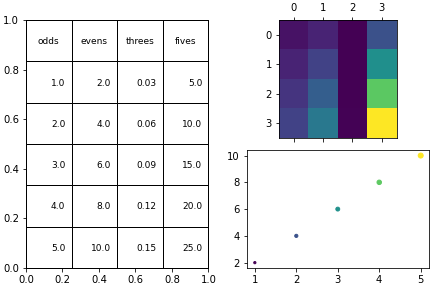
\includegraphics[width=.5\textwidth]{figures/intro/viz_same.png}
    \caption[]{Implicit in visualization is the assumption that these three representations of data are equivalent, specifically that the measurements within a variable and relations of the measurements of each variable are preserved. }
    \label{fig:viz_same}
\end{figure}

\section{Thesis statement}
We define a visualization as a transform from data to graphic that preserves the topology of the data and the properties of the measurement type. In fig~\ref{fig:viz_same}, we implicitly assume that the translation from table to heatmap has preserved the order of observations (the rows) and that the perceptually uniform sequential colormap has been applied such that the ordering relation on floats matches the ordering on the colormap (darker colors map to larger numbers). We also make this assumption about color in the scatter map, and that the translation to size and position on screen also respect the ordering on floats. In this work, we propose to mathematically describe the transform of data to visual space such that we can make explicit the implicit topology and types visualizations preserve. We then propose a new architecture for the Python visualization library Matplotlib \cite{hunterMatplotlib2DGraphics2007} based on these descriptions because the Matplolib artist layer is analogous to the transforms. 

\section{Notation \& Definitions}



\section{Background}
Bertin's proposed an organization of visual variables \cite{bertinIIPropertiesGraphic2011} 


\section{Library Review}
\subsection{Grammar of Graphics \& ggplot}
Specifies the end chart (graphic)
we want to specify the transformations ....
\begin{figure}
    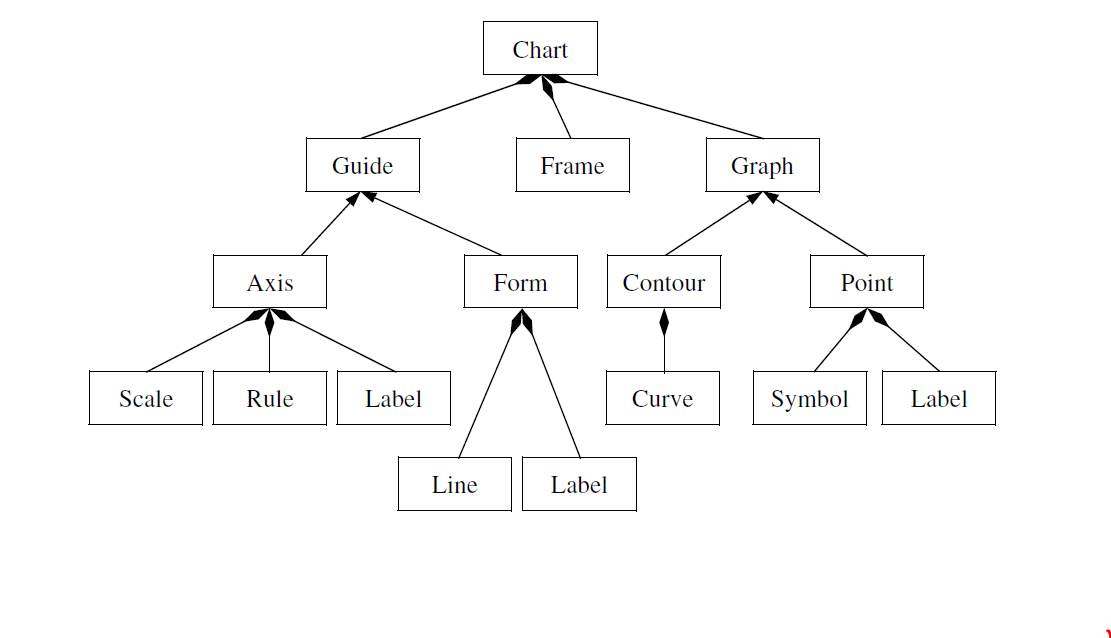
\includegraphics{figures/intro/grammar_chart_composition.png}
    \caption{page 10 (introduction)}
\end{figure}
\begin{figure}
    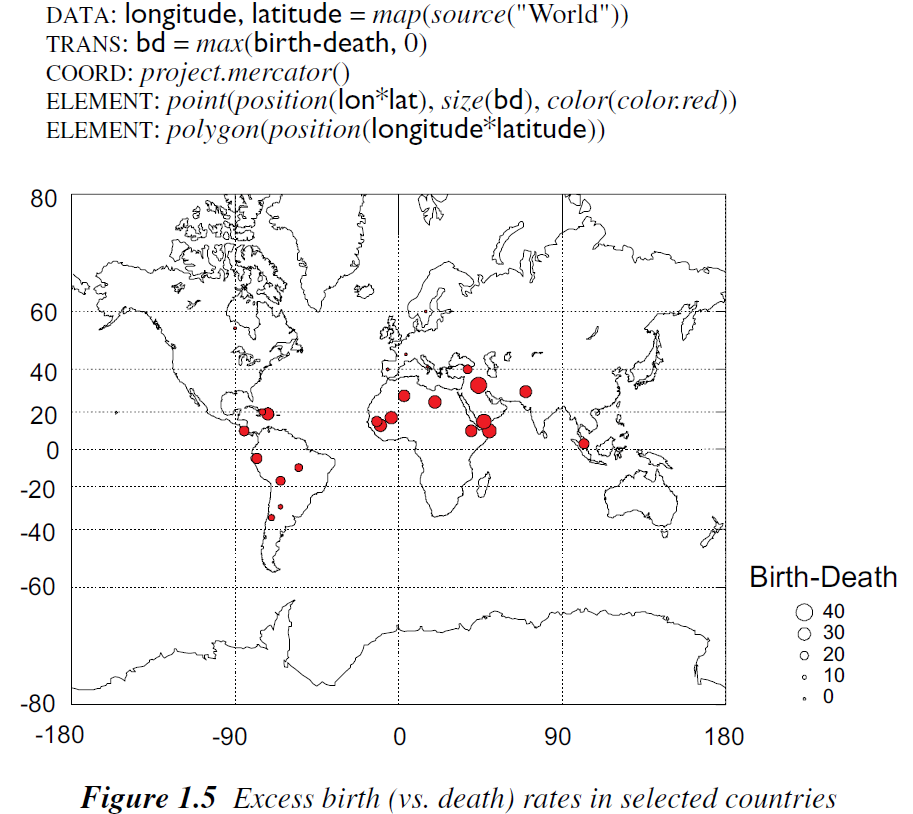
\includegraphics{figures/intro/grammar_example.png}
    \caption{Wilkenson decomposed a graphic into ...} 
\end{figure}
\cite{wilkinsonGrammarGraphicsStatistics2005}
charts - words 
    - instances of much more general objects (geometric primatives)
    - histogram =/= bar chart
graphics - statements 
expliceltly OO
    1. specification
        data - operations/computations
        trans - variable transforms (rank)
        scale - scale transforms
        coord - coordinate system
        element - marks and channels
        guide - meta elements - (axes, legends, etc)
    2. assembly - kinda what happens in artist (spec->something that can go to renderer) 
    3. display - rendering

How is our proposal different? seperation in spec between what's data, aesthetics, and render specific, and what part of the architecture owns those operations


ggplot - strictly hierarchal components (layers), matplotlib - transforms that mostly happen indepently 
"designing and producing statistical graphics is not an art" - ties in w/ difference between drawing program and visualization library, preservation of properties of measurement type and observation type

\cite{wickhamGgplot2ElegantGraphics2016}

history of viz - collins, friendly


Wilkenson suggests that the graphics pipeline could be implemented functionally but does not push it in any direction. 

ordering: processed before plotted, 
scales before stats, marks before channels
\begin{figure}
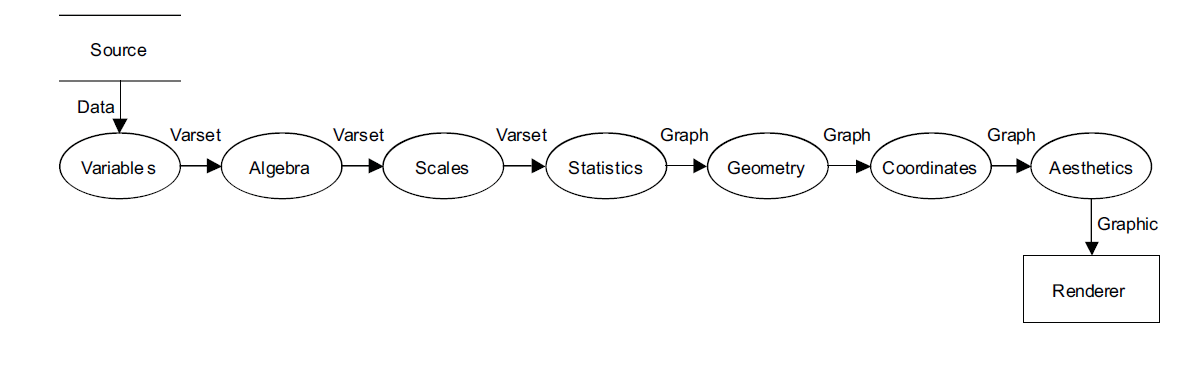
\includegraphics[]{figures/intro/gog_pathway.png}
\caption{Diagram of Grammar of Graphics stages of visualization. Fig 2.2 from chapter 2 of The Grammar of Graphics\cite{wilkinsonGrammarGraphics2005}}
\label{fig:gog_pathway}
\end{figure}
In grammar of graphics, as shown in figure~\ref{fig:gog_pathway} data is extracted from the database one variable at a time with an associated index (primary key). The algebra stage joins the variables to become the varset, which is a flat table where the columns are the variables/attributes, each row is an observation/item, and each cell contains a measurement \cite{munznerChDataAbstraction}. Wilkenson then describes the constraints of the measurement space for each variable through scales \cite{wilkinsonGrammarGraphics2005} with implicit assumptions of the data constraints. After this step, data is transformed computationally in service of the visualization. Some of the variables are then mapped into geometric marks (symbols) and are scaled (height, width) as appropriate. These mappings are then transformed into the coordinate system of the target graph. Then the aesthethic attributes (Bertin's retinal variables, also called channels) such as color or  texture) are applied. Finally

Wilkenson's thoughts on coherancy are equivalent to invariance but less? formally stated \dots

"To call these charts meainingul, defenders must falsify specific assumptions of GoG" \cite{wilkinsonMathematicalFoundationAnalytic2010}


gog implementationss:
\begin{enumerate}
    \item SPSS nViZn
    \item tableu
    \item ggplot
    \item protoviz\d3
    \item vega (interactive GoG)
\end{enumerate}


\printbibliography
\end{document}